\documentclass[10pt,a4paper]{article}
\usepackage{iftex}
\usepackage{amsmath,amssymb}
\ifPDFTeX
  \usepackage[T2A]{fontenc}
  \usepackage[utf8]{inputenc}
\else
  \usepackage{fontspec}
  \setmainfont{Times New Roman}
\fi
\usepackage[russian,english]{babel}
\usepackage[a4paper,margin=1.5cm,top=1.1cm,bottom=1.1cm]{geometry}
\usepackage{graphicx,booktabs,xcolor}
\usepackage[hidelinks]{hyperref}
\usepackage{enumitem}
\usepackage{titlesec}
\titleformat*{\section}{\normalsize\bfseries}
\titlespacing*{\section}{0pt}{0.6em}{0.2em}
\setlist{nosep,leftmargin=1.1em}
\setlength{\parskip}{0.25em}
\setlength{\parindent}{0pt}
\setlength{\emergencystretch}{2em}
\pagestyle{empty}
\definecolor{corange}{HTML}{EB6834}

\newcommand{\BasePPL}{14.06}
\newcommand{\NumMethods}{56}
\newcommand{\KMaxPlan}{12}
\newcommand{\kTwoWin}{3}
\newcommand{\kFiveWin}{6}
\newcommand{\kDoneWin}{12}
\newcommand{\dpplLastWin}{13.9\%}
\newcommand{\saveTwoWinShort}{1.7\%}
\newcommand{\saveTwoWinLong}{4.6\%}
\newcommand{\kvTwoWin}{10.6\%}
\newcommand{\saveFiveWinShort}{3.3\%}
\newcommand{\saveFiveWinLong}{9.3\%}
\newcommand{\kvFiveWin}{21.3\%}
\newcommand{\kTwoWinB}{3}
\newcommand{\kFiveWinB}{6}
\newcommand{\kDoneWinB}{8}
\newcommand{\dpplLastWinB}{5.7\%}
\newcommand{\saveTwoWinBShort}{0.6\%}
\newcommand{\saveTwoWinBLong}{2.3\%}
\newcommand{\kvTwoWinB}{10.6\%}
\newcommand{\saveFiveWinBShort}{1.3\%}
\newcommand{\saveFiveWinBLong}{4.5\%}
\newcommand{\kvFiveWinB}{21.3\%}
\newcommand{\kTwoWinS}{3}
\newcommand{\kFiveWinS}{6}
\newcommand{\kDoneWinS}{12}
\newcommand{\dpplLastWinS}{13.4\%}
\newcommand{\saveTwoWinSShort}{1.7\%}
\newcommand{\saveTwoWinSLong}{4.6\%}
\newcommand{\kvTwoWinS}{10.6\%}
\newcommand{\saveFiveWinSShort}{3.3\%}
\newcommand{\saveFiveWinSLong}{9.3\%}
\newcommand{\kvFiveWinS}{21.3\%}
\newcommand{\kTwoWinSB}{3}
\newcommand{\kFiveWinSB}{6}
\newcommand{\kDoneWinSB}{8}
\newcommand{\dpplLastWinSB}{5.5\%}
\newcommand{\saveTwoWinSBShort}{0.6\%}
\newcommand{\saveTwoWinSBLong}{2.3\%}
\newcommand{\kvTwoWinSB}{10.6\%}
\newcommand{\saveFiveWinSBShort}{1.3\%}
\newcommand{\saveFiveWinSBLong}{4.5\%}
\newcommand{\kvFiveWinSB}{21.3\%}
\newcommand{\kTwoHeadT}{—}
\newcommand{\kFiveHeadT}{1}
\newcommand{\kDoneHeadT}{12}
\newcommand{\dpplLastHeadT}{66.9\%}
\newcommand{\saveTwoHeadTShort}{—}
\newcommand{\saveTwoHeadTLong}{—}
\newcommand{\kvTwoHeadT}{—}
\newcommand{\saveFiveHeadTShort}{0.1\%}
\newcommand{\saveFiveHeadTLong}{0.4\%}
\newcommand{\kvFiveHeadT}{0.0\%}
\newcommand{\kTwoHeadTB}{—}
\newcommand{\kFiveHeadTB}{1}
\newcommand{\kDoneHeadTB}{8}
\newcommand{\dpplLastHeadTB}{32.2\%}
\newcommand{\saveTwoHeadTBShort}{—}
\newcommand{\saveTwoHeadTBLong}{—}
\newcommand{\kvTwoHeadTB}{—}
\newcommand{\saveFiveHeadTBShort}{0.1\%}
\newcommand{\saveFiveHeadTBLong}{0.2\%}
\newcommand{\kvFiveHeadTB}{0.0\%}
\newcommand{\kTwoOracle}{2}
\newcommand{\kFiveOracle}{6}
\newcommand{\kDoneOracle}{12}
\newcommand{\dpplLastOracle}{10.2\%}
\newcommand{\saveTwoOracleShort}{0.7\%}
\newcommand{\saveTwoOracleLong}{0.4\%}
\newcommand{\kvTwoOracle}{0.0\%}
\newcommand{\saveFiveOracleShort}{2.0\%}
\newcommand{\saveFiveOracleLong}{1.3\%}
\newcommand{\kvFiveOracle}{0.0\%}
\newcommand{\kTwoOracleB}{3}
\newcommand{\kFiveOracleB}{8}
\newcommand{\kDoneOracleB}{8}
\newcommand{\dpplLastOracleB}{4.8\%}
\newcommand{\saveTwoOracleBShort}{1.5\%}
\newcommand{\saveTwoOracleBLong}{1.3\%}
\newcommand{\kvTwoOracleB}{0.0\%}
\newcommand{\saveFiveOracleBShort}{4.1\%}
\newcommand{\saveFiveOracleBLong}{3.4\%}
\newcommand{\kvFiveOracleB}{0.0\%}
\newcommand{\kTwoRouted}{—}
\newcommand{\kFiveRouted}{3}
\newcommand{\kDoneRouted}{12}
\newcommand{\dpplLastRouted}{14.7\%}
\newcommand{\saveTwoRoutedShort}{—}
\newcommand{\saveTwoRoutedLong}{—}
\newcommand{\kvTwoRouted}{—}
\newcommand{\saveFiveRoutedShort}{2.4\%}
\newcommand{\saveFiveRoutedLong}{1.6\%}
\newcommand{\kvFiveRouted}{0.0\%}
\newcommand{\kTwoRoutedB}{3}
\newcommand{\kFiveRoutedB}{6}
\newcommand{\kDoneRoutedB}{8}
\newcommand{\dpplLastRoutedB}{6.0\%}
\newcommand{\saveTwoRoutedBShort}{3.9\%}
\newcommand{\saveTwoRoutedBLong}{3.2\%}
\newcommand{\kvTwoRoutedB}{0.0\%}
\newcommand{\saveFiveRoutedBShort}{7.7\%}
\newcommand{\saveFiveRoutedBLong}{6.5\%}
\newcommand{\kvFiveRoutedB}{0.0\%}
\newcommand{\kTwoSvd}{—}
\newcommand{\kFiveSvd}{1}
\newcommand{\kDoneSvd}{12}
\newcommand{\dpplLastSvd}{58.4\%}
\newcommand{\saveTwoSvdShort}{—}
\newcommand{\saveTwoSvdLong}{—}
\newcommand{\kvTwoSvd}{—}
\newcommand{\saveFiveSvdShort}{0.7\%}
\newcommand{\saveFiveSvdLong}{0.4\%}
\newcommand{\kvFiveSvd}{0.0\%}
\newcommand{\kTwoSvdB}{—}
\newcommand{\kFiveSvdB}{2}
\newcommand{\kDoneSvdB}{8}
\newcommand{\dpplLastSvdB}{34.6\%}
\newcommand{\saveTwoSvdBShort}{—}
\newcommand{\saveTwoSvdBLong}{—}
\newcommand{\kvTwoSvdB}{—}
\newcommand{\saveFiveSvdBShort}{2.1\%}
\newcommand{\saveFiveSvdBLong}{1.7\%}
\newcommand{\kvFiveSvdB}{0.0\%}
\newcommand{\kTwoWinRouted}{—}
\newcommand{\kFiveWinRouted}{2}
\newcommand{\kDoneWinRouted}{12}
\newcommand{\dpplLastWinRouted}{22.2\%}
\newcommand{\saveTwoWinRoutedShort}{—}
\newcommand{\saveTwoWinRoutedLong}{—}
\newcommand{\kvTwoWinRouted}{—}
\newcommand{\saveFiveWinRoutedShort}{2.7\%}
\newcommand{\saveFiveWinRoutedLong}{4.2\%}
\newcommand{\kvFiveWinRouted}{7.1\%}
\newcommand{\kTwoWinRoutedB}{2}
\newcommand{\kFiveWinRoutedB}{4}
\newcommand{\kDoneWinRoutedB}{6}
\newcommand{\dpplLastWinRoutedB}{5.9\%}
\newcommand{\saveTwoWinRoutedBShort}{3.0\%}
\newcommand{\saveTwoWinRoutedBLong}{3.7\%}
\newcommand{\kvTwoWinRoutedB}{7.1\%}
\newcommand{\saveFiveWinRoutedBShort}{6.0\%}
\newcommand{\saveFiveWinRoutedBLong}{7.3\%}
\newcommand{\kvFiveWinRoutedB}{14.2\%}
\newcommand{\kTwoWinSRouted}{—}
\newcommand{\kFiveWinSRouted}{—}
\newcommand{\kDoneWinSRouted}{—}
\newcommand{\dpplLastWinSRouted}{—}
\newcommand{\saveTwoWinSRoutedShort}{—}
\newcommand{\saveTwoWinSRoutedLong}{—}
\newcommand{\kvTwoWinSRouted}{—}
\newcommand{\saveFiveWinSRoutedShort}{—}
\newcommand{\saveFiveWinSRoutedLong}{—}
\newcommand{\kvFiveWinSRouted}{—}
\newcommand{\kTwoWinSRoutedB}{—}
\newcommand{\kFiveWinSRoutedB}{—}
\newcommand{\kDoneWinSRoutedB}{—}
\newcommand{\dpplLastWinSRoutedB}{—}
\newcommand{\saveTwoWinSRoutedBShort}{—}
\newcommand{\saveTwoWinSRoutedBLong}{—}
\newcommand{\kvTwoWinSRoutedB}{—}
\newcommand{\saveFiveWinSRoutedBShort}{—}
\newcommand{\saveFiveWinSRoutedBLong}{—}
\newcommand{\kvFiveWinSRoutedB}{—}
\newcommand{\kTwoWinSvd}{—}
\newcommand{\kFiveWinSvd}{1}
\newcommand{\kDoneWinSvd}{12}
\newcommand{\dpplLastWinSvd}{72.6\%}
\newcommand{\saveTwoWinSvdShort}{—}
\newcommand{\saveTwoWinSvdLong}{—}
\newcommand{\kvTwoWinSvd}{—}
\newcommand{\saveFiveWinSvdShort}{1.2\%}
\newcommand{\saveFiveWinSvdLong}{2.0\%}
\newcommand{\kvFiveWinSvd}{3.5\%}
\newcommand{\kTwoWinSvdB}{—}
\newcommand{\kFiveWinSvdB}{2}
\newcommand{\kDoneWinSvdB}{6}
\newcommand{\dpplLastWinSvdB}{28.1\%}
\newcommand{\saveTwoWinSvdBShort}{—}
\newcommand{\saveTwoWinSvdBLong}{—}
\newcommand{\kvTwoWinSvdB}{—}
\newcommand{\saveFiveWinSvdBShort}{2.5\%}
\newcommand{\saveFiveWinSvdBLong}{3.2\%}
\newcommand{\kvFiveWinSvdB}{7.1\%}
\newcommand{\dpplRoutedNaiveKTwo}{3.0\%}
\newcommand{\dpplRoutedNaiveKThree}{27.0\%}
\newcommand{\dpplRoutedNaiveKFour}{11.3\%}
\newcommand{\dpplRoutedNaiveBKTwo}{1.4\%}
\newcommand{\dpplRoutedNaiveBKThree}{2.0\%}
\newcommand{\dpplRoutedNaiveBKFour}{3.1\%}
\newcommand{\dpplWinRoutedNaiveKTwo}{3.2\%}
\newcommand{\dpplWinRoutedNaiveKThree}{29.6\%}
\newcommand{\dpplWinRoutedNaiveKFour}{13.1\%}
\newcommand{\dpplWinRoutedNaiveBKTwo}{—}
\newcommand{\dpplWinRoutedNaiveBKThree}{—}
\newcommand{\dpplWinRoutedNaiveBKFour}{—}
\newcommand{\dpplWinKTwo}{0.9\%}
\newcommand{\dpplWinKThree}{1.8\%}
\newcommand{\dpplWinKFour}{3.3\%}
\newcommand{\dpplWinBKTwo}{0.5\%}
\newcommand{\dpplWinBKThree}{1.5\%}
\newcommand{\dpplWinBKFour}{2.8\%}
\newcommand{\dpplWinSKTwo}{0.9\%}
\newcommand{\dpplWinSKThree}{1.8\%}
\newcommand{\dpplWinSKFour}{3.3\%}
\newcommand{\dpplWinSBKTwo}{0.5\%}
\newcommand{\dpplWinSBKThree}{1.4\%}
\newcommand{\dpplWinSBKFour}{2.8\%}
\newcommand{\dpplHeadTKTwo}{7.4\%}
\newcommand{\dpplHeadTKThree}{23.7\%}
\newcommand{\dpplHeadTKFour}{19.2\%}
\newcommand{\dpplHeadTBKTwo}{6.3\%}
\newcommand{\dpplHeadTBKThree}{9.4\%}
\newcommand{\dpplHeadTBKFour}{8.3\%}
\newcommand{\dpplOracleKTwo}{1.2\%}
\newcommand{\dpplOracleKThree}{2.2\%}
\newcommand{\dpplOracleKFour}{2.9\%}
\newcommand{\dpplOracleBKTwo}{0.9\%}
\newcommand{\dpplOracleBKThree}{1.4\%}
\newcommand{\dpplOracleBKFour}{2.1\%}
\newcommand{\dpplRoutedKTwo}{3.0\%}
\newcommand{\dpplRoutedKThree}{4.7\%}
\newcommand{\dpplRoutedKFour}{6.4\%}
\newcommand{\dpplRoutedBKTwo}{1.4\%}
\newcommand{\dpplRoutedBKThree}{1.7\%}
\newcommand{\dpplRoutedBKFour}{3.0\%}
\newcommand{\dpplSvdKTwo}{8.1\%}
\newcommand{\dpplSvdKThree}{12.8\%}
\newcommand{\dpplSvdKFour}{17.5\%}
\newcommand{\dpplSvdBKTwo}{4.0\%}
\newcommand{\dpplSvdBKThree}{7.6\%}
\newcommand{\dpplSvdBKFour}{12.1\%}
\newcommand{\dpplWinRoutedKTwo}{3.2\%}
\newcommand{\dpplWinRoutedKThree}{5.2\%}
\newcommand{\dpplWinRoutedKFour}{7.5\%}
\newcommand{\dpplWinRoutedBKTwo}{1.3\%}
\newcommand{\dpplWinRoutedBKThree}{2.3\%}
\newcommand{\dpplWinRoutedBKFour}{3.9\%}
\newcommand{\dpplWinSRoutedKTwo}{—}
\newcommand{\dpplWinSRoutedKThree}{—}
\newcommand{\dpplWinSRoutedKFour}{—}
\newcommand{\dpplWinSRoutedBKTwo}{—}
\newcommand{\dpplWinSRoutedBKThree}{—}
\newcommand{\dpplWinSRoutedBKFour}{—}
\newcommand{\dpplWinSvdKTwo}{8.7\%}
\newcommand{\dpplWinSvdKThree}{14.4\%}
\newcommand{\dpplWinSvdKFour}{21.3\%}
\newcommand{\dpplWinSvdBKTwo}{4.4\%}
\newcommand{\dpplWinSvdBKThree}{9.0\%}
\newcommand{\dpplWinSvdBKFour}{14.9\%}
\newcommand{\InfoB}{На Qwen3-1.7B (тоже 28 слоёв, вдвое шире; посчитано до $k=8$): окно 64 + сток — 3 слоя при $\le 2\,\%$ и 6 при $\le 5\,\%$; M-O4 — 3 и 6; отбор по активациям — 3 и 8.}


\begin{document}
\selectlanguage{russian}

{\Large\bfseries Детерминированная замена первых слоёв языковой модели}\\[0.15em]
{\large Зачем это нужно, как мы это измеряем и сколько слоёв можно заменить}

\section*{Зачем}

Языковая модель (здесь "--- Qwen3-0.6B и Qwen3-1.7B, а также SmolLM2-1.7B
семейства Llama) состоит из 28 (24) одинаково устроенных слоёв, и каждый токен текста проходит через все. Первый слой стоит столько же,
сколько последний, хотя делает более простую работу: склеивает части слов,
смотрит на соседние токены и пунктуацию, запоминает частые сочетания.
Мы проверяем, можно ли \textbf{первые слои заменить явными дешёвыми
алгоритмами}, которые строятся из весов готовой модели и небольшого корпуса
текста за минуты "--- без обучения градиентным спуском и без случайности
(отсюда «детерминированная» замена). Если это удаётся, мы получаем:
\begin{itemize}
  \item \textbf{скорость и память} "--- меньше операций на токен и меньше кэша
    ключей-значений на длинном контексте;
  \item \textbf{понимание модели} "--- если слой заменён явной формулой почти
    без изменения ответов модели, эта формула и есть проверяемое объяснение
    того, что слой делает;
  \item \textbf{воспроизводимость} "--- тот же вход даёт тот же выход, а ошибку
    замены можно измерить и разобрать по слоям.
\end{itemize}

\section*{Как устроена модель и что именно мы меняем}

\begin{center}
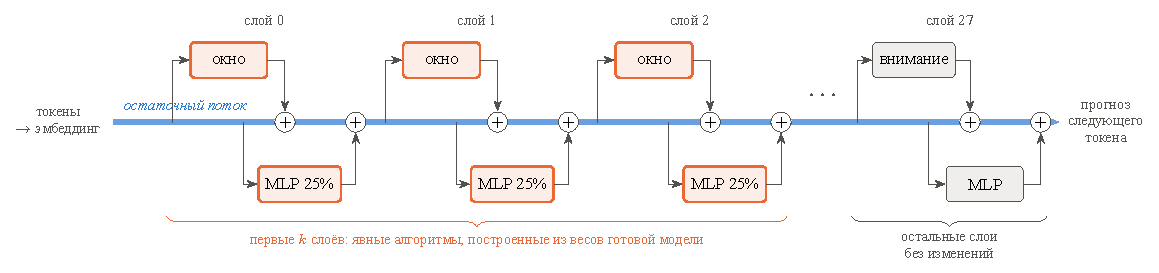
\includegraphics[width=\linewidth]{figs/arch_A.pdf}
\end{center}

Текст режется на токены, каждый токен превращается в вектор из 1024 чисел.
Дальше этот вектор едет по \emph{остаточному потоку} (синяя линия) через
28 слоёв: каждый слой читает вектор, вычисляет поправку и \emph{прибавляет} её
к потоку (знаки «$+$»). В слое два блока. \textbf{Внимание} "--- единственное
место, где токен получает информацию от предыдущих токенов: он сравнивает себя
с каждым из них, назначает веса и собирает взвешенную сумму. \textbf{MLP}
обрабатывает каждый токен отдельно: 3072 «нейронов», каждый проверяет свой
признак и, если признак сработал, добавляет к потоку свой вектор. На коротком
контексте MLP "--- около двух третей умножений слоя; внимание дорожает с длиной
контекста $T$, потому что сравнивает токен со всеми предыдущими.

Мы берём готовую модель и заменяем первые $k$ слоёв (оранжевые блоки), остальные
$28-k$ не трогаем. Внимание заменяется \emph{окном}: токен смотрит только на
64 предыдущих и на самый первый токен текста (его называют «стоком», модель
использует его как «никуда не смотреть»). MLP заменяется подмножеством нейронов:
наш метод M-O4 по вектору токена предсказывает, какие 25\,\% нейронов сработают,
и считает только их; SVD-LLM из литературы вместо этого сжимает матрицы
нейронов вдвое. Все параметры замены "--- поправки, предиктор, выбор нейронов "---
вычисляются по явным формулам (метод наименьших квадратов) из весов модели и
128 тыс. токенов калибровочного текста. Слои заменяются по очереди, и каждая
следующая замена калибруется с учётом ошибки предыдущих.

\section*{Как измеряем}

\begin{itemize}
  \item \textbf{Данные} "--- WikiText (Merity и др., 2017; Salesforce Research): статьи
    английской Википедии категорий Good/Featured. Калибровка "--- 256 случайных окон по 512
    токенов (128 тыс.) из WikiText-103 train (103 млн слов); оценка "--- первые 32 окна по 1024
    токена из WikiText-2 test; наборы не пересекаются. Бенчмарки "--- из lm-evaluation-harness.
  \item \textbf{Perplexity (PPL)} "--- «насколько модель удивлена текстом»:
    экспонента средней ошибки предсказания следующего токена на 32 тыс. токенов
    WikiText-2. У исходной модели \BasePPL; меньше "--- лучше. Главная метрика
    записки "--- \emph{рост} PPL после замены. Порог 2\,\% считаем «практически
    без потерь» (шум измерения "--- десятые доли процента), 5\,\% "--- «заметно, но приемлемо».
  \item \textbf{KL-расхождение} "--- насколько распределение вероятностей
    следующего токена у модели с заменой отличается от исходной модели
    ($0$ "--- совпадает). Точнее PPL: сравнивает с моделью, а не с текстом.
  \item \textbf{Совпадение top-1} "--- доля позиций, где обе модели называют один
    и тот же самый вероятный следующий токен.
  \item \textbf{Бенчмарки} "--- 7 стандартных задач (LAMBADA, HellaSwag, ARC,
    PIQA, WinoGrande, MMLU: вопросы на знания и здравый смысл) на подвыборках по
    200 примеров.
  \item \textbf{Стоимость} "--- доля умножений на токен во всей модели,
    которую экономит замена, для контекста $T=2048$ и $8192$, и доля
    сэкономленного кэша ключей-значений.
\end{itemize}

\clearpage
\section*{Сколько слоёв можно заменить}

\begin{center}
\footnotesize\setlength{\tabcolsep}{4.5pt}
\begin{tabular}{llcccc}
\toprule
Метод & Что заменено & \multicolumn{2}{c}{Сколько слоёв $k$: Qwen3-0.6B / 1.7B / SmolLM2} & \multicolumn{2}{c}{Экономия умножений (0.6B)} \\
 & & при $\Delta$PPL$\le$2\% & при $\Delta$PPL$\le$5\% & при $k_{2\%}$ & при $k_{5\%}$ \\
 & & & & \scriptsize $T{=}2048$ / $8192$ & \scriptsize $T{=}2048$ / $8192$ \\
\midrule
Окно 64 + сток & внимание & 3 / 3 / 1 & 6 / 6 / 2 & 1.7\% / 4.6\% & 3.3\% / 9.3\% \\
\textbf{Окно 64 + массивные стоки} & внимание & 3 / 3 / 3 & 6 / 6 / 8 & 1.7\% / 4.6\% & 3.3\% / 9.3\% \\
\textbf{O1: половина голов → позиционное ядро} & внимание & — / — / — & 1 / 1 / 1 & — & 0.1\% / 0.4\% \\
Отбор 25\% нейронов по активациям (Deja Vu) & MLP & 2 / 3 / 4 & 6 / 8 / 8 & 0.7\% / 0.4\% & 2.0\% / 1.3\% \\
\textbf{M-O4: предиктор нейронов, 25\%} & MLP & — / 3 / — & 3 / 6 / — & — & 2.4\% / 1.6\% \\
SVD-LLM, ранг 50\% & MLP & — / — / — & 1 / 2 / — & — & 0.7\% / 0.4\% \\
\textbf{Окно 64 + сток + M-O4} & блок & — / 2 / — & 2 / 4 / — & — & 2.7\% / 4.2\% \\
\textbf{Окно 64 + массивные стоки + M-O4} & блок & … / … / — & … / … / — & — & — \\
Окно 64 + сток + SVD-LLM & блок & — / — / — & 1 / 2 / — & — & 1.2\% / 2.0\% \\
\bottomrule
\end{tabular}

\end{center}
\vspace{-0.3em}
{\footnotesize Жирным "--- наши методы; остальные "--- из литературы. $k$ "--- наибольшее число
первых слоёв, при котором порог выполняется для всех $k' \le k$; проверены
$k = 1, 2, 3, 4, 6, 8, 12$ (1.7B и SmolLM2 "--- до 8; «…» "--- ещё считается; «$\ge k$» "--- кривая
досчитана до $k$ и порог ещё не нарушен). Экономия умножений дана для 0.6B, у 1.7B доли те же с
точностью до долей процента.\par}

\begin{center}
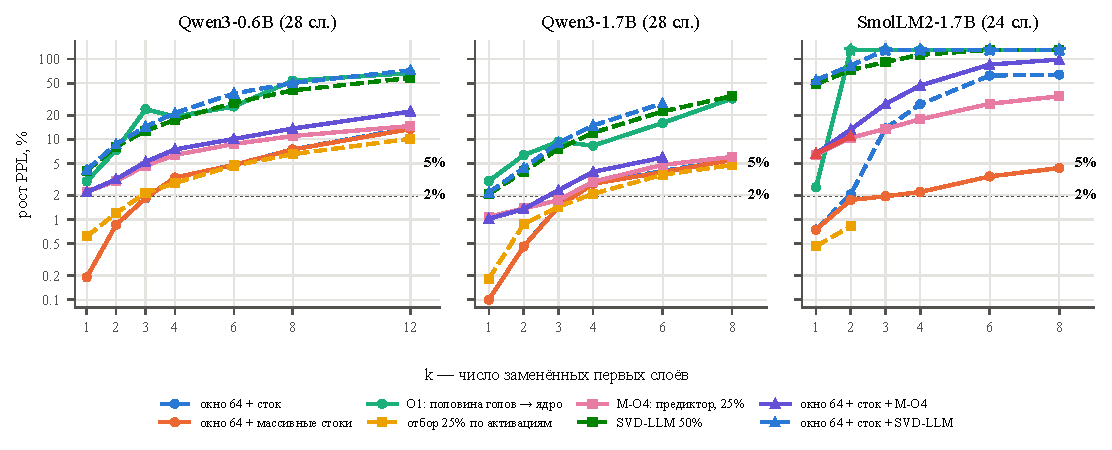
\includegraphics[width=0.8\linewidth]{fig_howmany.pdf}
\end{center}

\begin{enumerate}
  \item \textbf{Внимание первых слоёв заменяется почти даром.} Окно 64 + сток:
    \kTwoWin{} слоя при росте PPL $\le 2\,\%$ и \kFiveWin{} при $\le 5\,\%$;
    на семи бенчмарках отличия от исходной модели в пределах $\pm 2$ пунктов,
    т.\,е. шума. Но экономия умножений мала: \saveTwoWinShort{} при $T=2048$ и
    \saveTwoWinLong{} при $T=8192$ для $k=\kTwoWin$ (\saveFiveWinShort{} и
    \saveFiveWinLong{} для $k=\kFiveWin$). Главный выигрыш "--- память: кэш
    ключей-значений в заменённых слоях сокращается с $T$ до 64 позиций, это
    \kvTwoWin{} ($k=\kTwoWin$) и \kvFiveWin{} ($k=\kFiveWin$) всего кэша при $T=8192$.
    Ошибка окна растёт плавно: даже при $k=\kDoneWin$ (почти половина слоёв) PPL выше
    исходной лишь на \dpplLastWin. \InfoB
  \item \textbf{MLP первых слоёв сжимается дорого.} Лучшее из реализуемого "---
    наш M-O4 (предиктор выбирает 25\,\% нейронов до их вычисления): $\le 5\,\%$
    до $k=\kFiveRouted$ (рост \dpplRoutedKThree{} при $k=3$); SVD-LLM (ранг 50\,\%) "---
    $k=\kFiveSvd$. Отбор по готовым активациям (Deja Vu: все нейроны вычисляются,
    слабые отбрасываются перед последней матрицей) держит $\le 5\,\%$ до
    $k=\kFiveOracle$, но экономит лишь треть MLP. Комбинации «окно + MLP»
    наследуют ошибку MLP-части.
  \item \textbf{Ответ на вопрос.} Без потерь ($\le 2\,\%$) можно заменить
    первые \kTwoWin{} слоя внимания; для MLP без потерь "--- только \kTwoOracle{} слоя
    и только отбором по готовым активациям. С допуском 5\,\% "--- \kFiveWin{} слоёв
    внимания или \kFiveWinRouted{} слоя целиком (окно + M-O4). Выигрыш в скорости
    при этом "--- единицы процентов: первые три слоя "--- это $3/28\approx 11\,\%$
    модели, а внимание на коротком контексте "--- малая часть слоя. Выиграть в
    качестве (PPL ниже исходной) не удалось ни одному методу.
  \item \textbf{Ловушка калибровки.} Наивно откалиброванный M-O4 давал
    \dpplRoutedNaiveKThree{} при $k=3$ против \dpplRoutedNaiveKTwo{} при $k=2$ "---
    обрыв на слое, где возникает сток. Причина "--- 1.6\,\% окон калибровки (около 4 из 256),
    где сток возникает не на позиции~0, а на токене вроде «0» или «=»: выход MLP слоя~2
    для него имеет норму 7\,059 при медиане 4.9, такие строки захватывают метод наименьших
    квадратов, и ошибка ложится в каналы массивной активации у всех токенов. Управляемый
    эксперимент: 0, 1, 4, 16 отравленных окон дают 4.2, 4.2, 23.9 и 379\,\%; Qwen3-1.7B
    иммунна (1.6--1.7\,\% при любой дозе). Исключение таких строк снимает обрыв:
    \dpplRoutedKThree{} при $k=3$.
\end{enumerate}


\clearpage
\section*{Что ещё показали эксперименты}

\textbf{Карта заменяемости и априорный критерий.} Мы заменяли каждый из 28 слоёв
\emph{по отдельности} (внимание "--- окном, MLP "--- отбором 25\,\% нейронов) и измеряли
KL к исходной модели. Внимание везде заменяется легко, кроме слоя~3, где возникает
сток, и последнего слоя; MLP, наоборот, незаменим именно в первых шести слоях и
становится заменимым к концу модели. Ошибку замены можно предсказать \emph{до}
замены по статистикам самого слоя: доля веса внимания вне окна предсказывает
KL окна, локальная ошибка отбора нейронов относительно нормы остаточного потока
"--- KL замены MLP (ранговая корреляция Спирмена 0.91--0.97 на обеих моделях).
Критерий подогнан на 0.6B и без изменений применён к 1.7B: план из $m$ замен с
наименьшей предсказанной ошибкой даёт KL в 10--15 раз ниже, чем замена первых
слоёв подряд (рис. ниже). План сам уводит замену из начала модели в хвост: MLP
слоёв 23--27 и внимание слоя~0.

\begin{center}
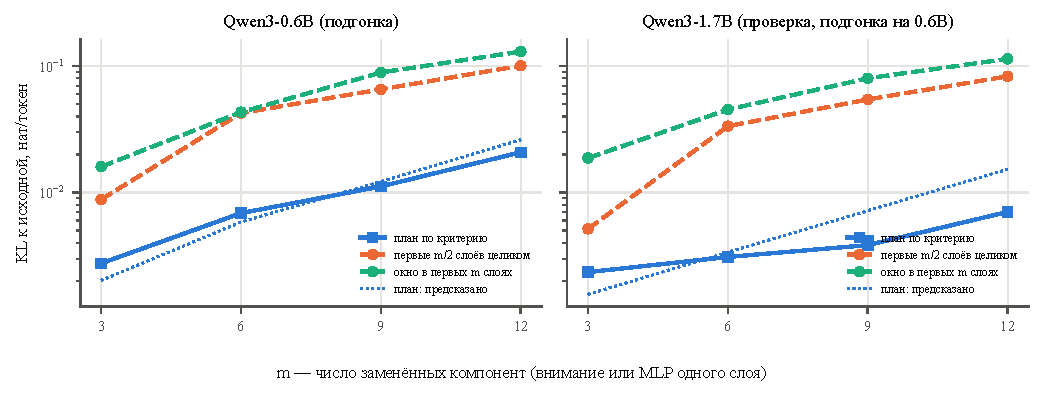
\includegraphics[width=0.78\linewidth]{../figures/planner.pdf}
\end{center}

\textbf{Почему MLP первых слоёв незаменим.} В слоях 0--5 активны 60--74\,\%
нейронов (в поздних "--- 40\,\%), выход MLP составляет 0.45--0.72 нормы остаточного
потока (в поздних "--- 0.2--0.4), а вклад распределён по нейронам равномерно:
концентрация вклада в 25\,\% сильнейших нейронов коррелирует с ошибкой замены на
$-0.92$. Ранние MLP пишут большие, плотные и высокоранговые поправки, особенно при
сборке слов из кусков токенов; «малое подмножество нейронов» для них не существует.

\textbf{Нейроны стока.} Массивную активацию первого токена (норма около 7\,000)
создают 5 нейронов MLP слоя~2 у 0.6B и 1 нейрон у 1.7B (90--94\,\% вклада).
Удаление их всюду ломает модель: $+54\,\%$ и $+231\,\%$ PPL; удаление на всех
позициях, кроме первой, "--- $+0.3\,\%$ и $0.0\,\%$. Это значит, что любая замена
слоя~2 обязана считать первую позицию точно или сохранять эти нейроны явно;
в наших методах первая позиция считается точно.

\textbf{Обменный курс.} Все работающие замены 0.6B ложатся на одну линию
«1\,\% PPL за 1\,\% сэкономленных умножений» (контекст 2048); у 1.7B курс в
2.5 раза лучше "--- около 0.4\,\% PPL за процент. Методы с ошибочным критерием
выбора (SVD-LLM, отбор по косинусной близости состояний, как в ShortGPT) лежат в
разы выше линии. Если курс продолжает улучшаться с размером, замена слоёв станет
выгодной на моделях 4B--32B "--- это проверяется на GPU.

\textbf{Домен калибровки.} Окно не калибруется и переносится без потерь
(1.2\,\% на pile-10k против 1.8\,\% на WikiText-2). Калиброванные замены MLP
переобучаются под корпус: робастный M-O4 при калибровке на WikiText-103 стоит
4.7\,\% на WikiText-2 и 16.4\,\% на pile-10k. Калибровка на смеси доменов
выравнивает ошибку (8.6 и 8.0\,\%); текст, сгенерированный самой моделью,
не помогает.

\textbf{Второе семейство.} На SmolLM2-1.7B (архитектура Llama, 24 слоя, без QK-нормализации,
связанные эмбеддинги) сток привязан не к позиции, а к токену: один нейрон MLP слоя~1 создаёт
массивную активацию на слове «the» в любой позиции, и поздние слои смотрят на эти токены как
на стоки. Отсюда два правила: при замене MLP нейроны стока сохраняются явно (M-O4 при $k=2$:
123\,\% $\to$ 11\,\%), при замене внимания окно хранит массивные ключи ($k=8$: 64\,\% $\to$ 4.4\,\%
при неизменных бенчмарках). Внимание при этом заменяется так же, как у Qwen3 (3 слоя при 2\,\%,
8 при 5\,\%), а MLP первых слоёв "--- заметно хуже (M-O4 6\,\% уже при $k=1$, хотя
оракульный отбор 25\,\% нейронов держит $\le 4\,\%$ до $k=8$: узкое место "--- предиктор);
блок «окно с массивными стоками + M-O4» стоит столько же, сколько один M-O4 (19\,\% при $k=4$
против 47\,\% у блока с позиционным стоком); планировщик по
критерию переносится (6 компонент: 2.6\,\% против 16--62\,\% у префиксов), критерий для MLP "---
слабее (корреляция $-0.25$ против $-0.91$). Llama-3.2-1B считается.

\section*{Что не работает}
\begin{itemize}
  \item \textbf{Быстрое внимание из литературы без переобучения.} Performer
    (случайные признаки) и линейное внимание ломают модель: нормы ключей в Qwen3
    равны 30--60, а эти приближения устойчивы лишь при нормах порядка единицы.
  \item \textbf{Замена голов позиционным ядром (O1).} Даже один слой даёт $+3\,\%$:
    в первых слоях внимание зависит от содержания токенов, а не только от расстояния.
  \item \textbf{Окно с «хвостом»} (наш O5: окно плюс грубая сводка далёких токенов)
    не лучше обычного окна.
\end{itemize}

\section*{Ограничения}
Экономия посчитана по числу умножений: наша реализация окна на чистом PyTorch
медленнее встроенного ядра, ускорение требует специального ядра. Калиброванные
замены MLP переобучаются под домен калибровки (вне домена ошибка втрое выше),
лечится смесью корпусов. Бенчмарки главных столбцов на 1000 примерах
($\pm$1 пункт), остальных "--- на 200 ($\pm$2.5); интервалы для PPL узкие.

\end{document}
